\documentclass[table]{beamer}
\usepackage[utf8]{inputenc}
\DeclareGraphicsExtensions{.pdf}
\title{Vakaa avioliitto -ongelma}
\subtitle{Kandidaatintutkielman esitelmä}
\author{Anis Moubarik}
\date{}
\begin{document}
	\frame{\titlepage}
	\begin{frame}
		\frametitle{Johdanto}
		\fontsize{18pt}{7.2}\selectfont
		\begin{itemize}
			\item Ongelman alkuperä
			\item Ongelman kuvaus
			\item Avioliitto ja avioliittopeli
		\end{itemize}
	\end{frame}
	\begin{frame}
    \frametitle{Pari ja pariutukset}
    \fontsize{14pt}{7.2}\selectfont
    \begin{itemize}
		\item Paria merkitään seuraavasti $(m, n) \in M \times N$ missä $m \in M, n \in N$.
		\item  Pariutus on parien joukko avioliittopelissä.
    \end{itemize}
    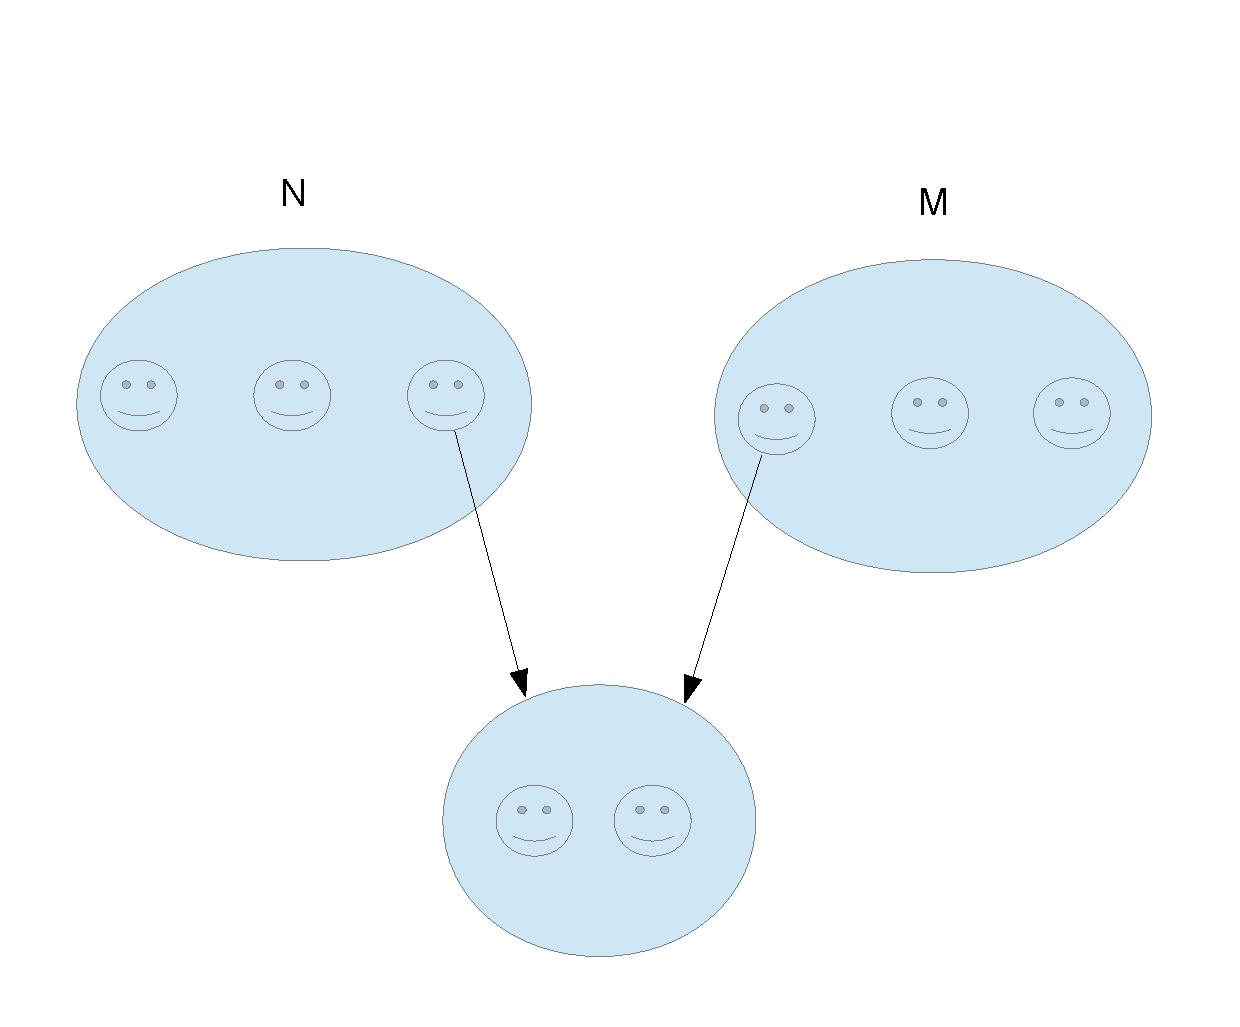
\includegraphics[scale=0.42]{vakaa1}
  \end{frame}
  \begin{frame}
  	\frametitle{Mieltymykset}
  	\begin{table}[h!]
	\begin{tabular}{ l | *{2}{c} r }
	 &  \\
	 \hline
 	 $m_{1}$ & $n_{2}$ & $n_{1}$ & $n_{3}$ \\
 	 $m_{2}$ & $n_{1}$ & $n_{2}$ & $n_{3}$ \\
 	 $m_{3}$ & $n_{3}$ & $n_{1}$ & $n_{2}$ \\
	\end{tabular}
	\caption{Miesten mieltymykset}
	\end{table}
	\begin{table}[h!]
	\begin{tabular}{ l | *{2}{c} r }
	 &  \\
	 \hline
 	 $n_{1}$ & $m_{1}$ & $m_{2}$ & $m_{3}$ \\
 	 $n_{2}$ & $m_{2}$ & $m_{1}$ & $m_{3}$ \\
 	 $n_{3}$ & $m_{3}$ & $m_{2}$ & $m_{1}$ \\
	\end{tabular}
	\caption{Naisten mieltymykset}
	\end{table}
  \end{frame}
  \begin{frame}
  	\frametitle{Pariutusten notaatio}
  	\fontsize{14pt}{7.2}\selectfont
  	Pariutus $\mu$ on joukko $\mu \subseteq M \times N$, joka tulkittuna funktioksi on injektio $\mu: M \rightarrow N$. \\Alkion $m$ paria pariutuksessa $\mu$ merkitään $p_{\mu}(m)$. \\Mieltymyksiä voidaan kuvailla transitiivisella relaatiolla, esim. $n_1 >_{m} n_2$, $n_1 \in N$ $n_2 \in N$.
  \end{frame}
  \begin{frame}
    \frametitle{Vakaat pariutukset}
    \fontsize{14pt}{7.2}\selectfont
    \begin{itemize}
		\item Ongelma on löytää vakaa pariutus joukoille $M$ ja $N$.
		\item Pariutus on vakaa, kun meillä ei ole kahta vastakkaisen sukupuolen henkilöä, jotka olisivat mielummin pari keskenään kuin pitäisivät nykyisen parinsa. 
    \end{itemize}
    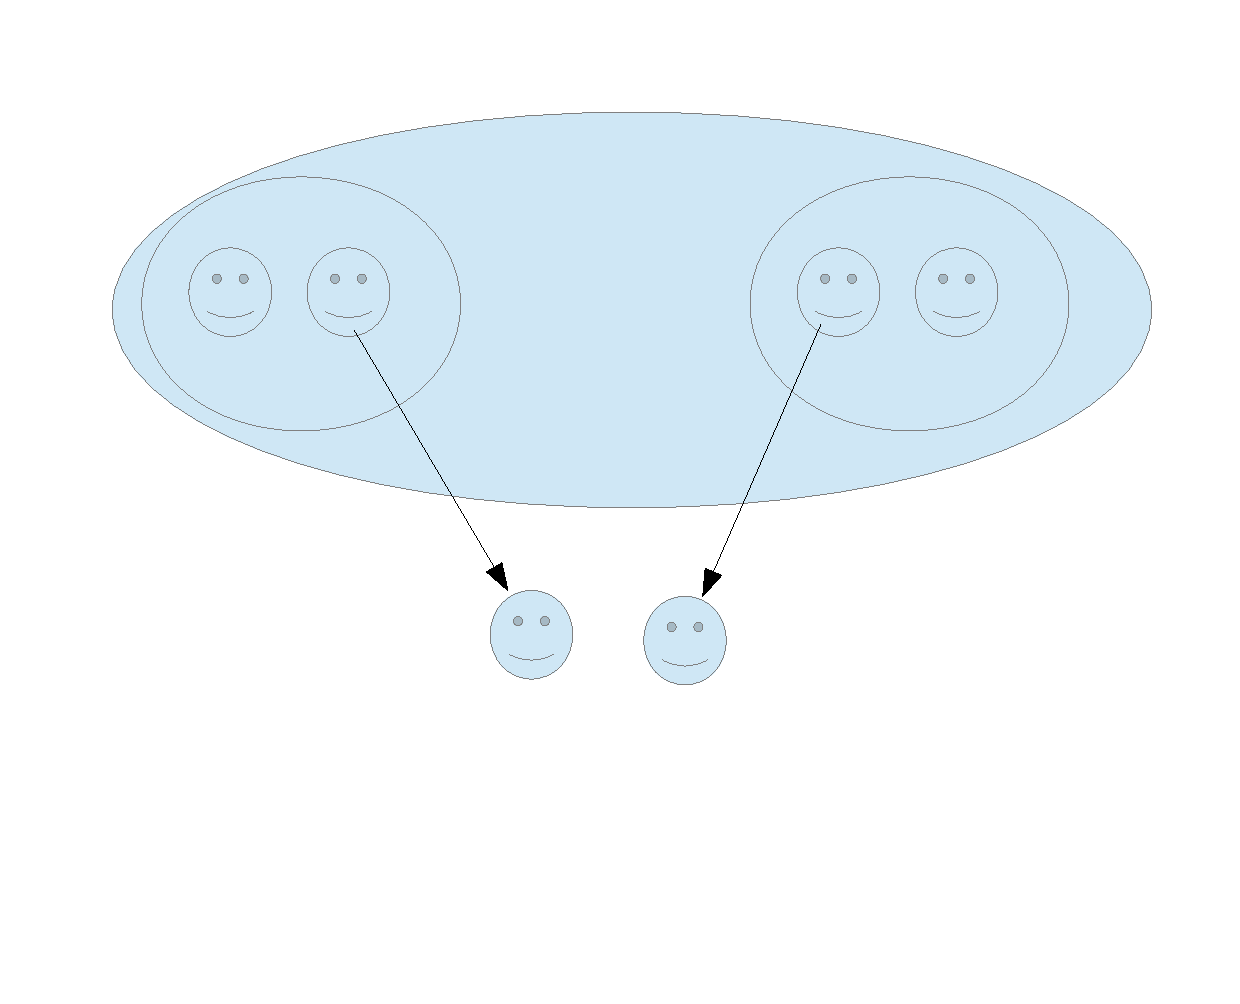
\includegraphics[scale=0.5]{epavakaa}
  \end{frame}
  \begin {frame}
  	\frametitle{Esteparin määritelmä}
  	\fontsize{18pt}{7.2}\selectfont
  	Pariutus $\mu$ on vakaa, jos ei ole olemassa miestä $m_{1}$ ja naista  $n_{2}$, jolle
  	\begin{enumerate}
  		\item $n_2 >_{m_{1}} p_{\mu}(m_1)$, ja
  		\item $m_1 >_{n_{2}} p_{\mu}(n_2)$
  	\end{enumerate}
  \end{frame}
  \begin{frame}
    \frametitle{Gale--Shapley-algoritmi}
    \begin{enumerate}
	\item Miehet aloittavat kosimalla mieltymyksiltään parasta naista.
	\item Naiset hylkäävät kaikki paitsi parhaiten sijoitetun miehen.
	\item Nainen ei hyväksy miestä vaan odottaa, jos parempi mies kosisi häntä
	\item Hylätyt miehet kosivat mieltymyksiltään toisiksi parasta naista.
	\item Naiset hylkäävät kaikki paitsi parhaan vaihtoehdon
	\item Niin kauan kuin joku naisista ei ole saanut kosintaa, tulee hylkäyksiä ja uusia kosintoja. Lopuksi jokaista naista on kosittu, koska mies ei voi kuin kerran kosia samaa naista.
	\item Viimeinen nainen on saanut kosinnan ja kosimisvaihe on päättynyt. Jokainen nainen hyväksyy langan päässä olevan kosijan
\end{enumerate}
  \end{frame}
    \begin{frame}
  	\frametitle{Gale--Shapley-algoritmi 2.}
  	\begin{table}[h!]
	\begin{tabular}{ l | *{2}{c} r }
	 &  \\
	 \hline
 	 $m_{1}$ & \cellcolor{blue!50}$n_{2}$ & $n_{1}$ & $n_{3}$ \\
 	 $m_{2}$ & \cellcolor{blue!50}$n_{1}$ & $n_{2}$ & $n_{3}$ \\
 	 $m_{3}$ & \cellcolor{blue!50}$n_{3}$ & $n_{1}$ & $n_{2}$ \\
	\end{tabular}
	\caption{Miesten parit}
	\end{table}
	\begin{table}[h!]
	\begin{tabular}{ l | *{2}{c} r }
	 &  \\
	 \hline
 	 $n_{1}$ & $m_{1}$ & \cellcolor{pink!50}$m_{2}$ & $m_{3}$ \\
 	 $n_{2}$ & $m_{2}$ & \cellcolor{pink!50}$m_{1}$ & $m_{3}$ \\
 	 $n_{3}$ & \cellcolor{pink!50}$m_{3}$ & $m_{2}$ & $m_{1}$ \\
	\end{tabular}
	\caption{Naisten parit}
	\end{table}
  \end{frame}
  \begin{frame}
  	\frametitle{Vakaitten pariutuksien joukko}
  	\fontsize{14pt}{7.2}\selectfont
  	\begin{itemize}
  		\item Gale--Shapley tuottaa yhden vakaan pariutuksen, niitä voi olla kuitenkin enemmän.
  		\item Niitä voi olla enintään eksponentiaalinen määrä.
  	\end{itemize}
  \end{frame}
  \begin{frame}
  	\frametitle{Erisuuruiset joukot}
  	\fontsize{14pt}{7.2}\selectfont
  	\begin{itemize}
  		\item Erisuuruisten joukkojen tapauksessa oletamme, että henkilö haluaa parin mielummin kuin olla yksin.
  		\item Isomman joukon alkioista jää parittomaksi pienemmän ja isomman joukon erotuksen verran alkioita.	
  	\end{itemize}
  \end{frame}
  \begin{frame}
  	\frametitle{Pareista kieltäytyminen}
  	\fontsize{16pt}{7.2}\selectfont
  	\begin{itemize}
  		\item Parin on mahdollista ilmoittaa, että yksi tai useampi pari ei kelpaa hänelle.
  		\item Pariutus voi olla osittainen.
  	\end{itemize}
  \end{frame}
  \begin{frame}
  	\frametitle{Sovellukset}
  	\fontsize{16pt}{7.2}\selectfont
  	\begin{itemize}
  		\item Elinluovutus
  		\item Koulujen valinnat
  		\item Lääketieteen opiskelijat ja opetussairaalat
  	\end{itemize}
  \end{frame}
\end{document}